\subsection{Efficiency and Angular Resolution}%
\label{sub:Efficiency_AR}

\begin{frame}{Efficiency and Angular Resolution}
    \begin{equation*}
        \eff = \frac{n_\text{reco}}{n_\text{total}}
    \end{equation*}
    \begin{columns}
        \begin{column}{0.48\textwidth}
            \centering
            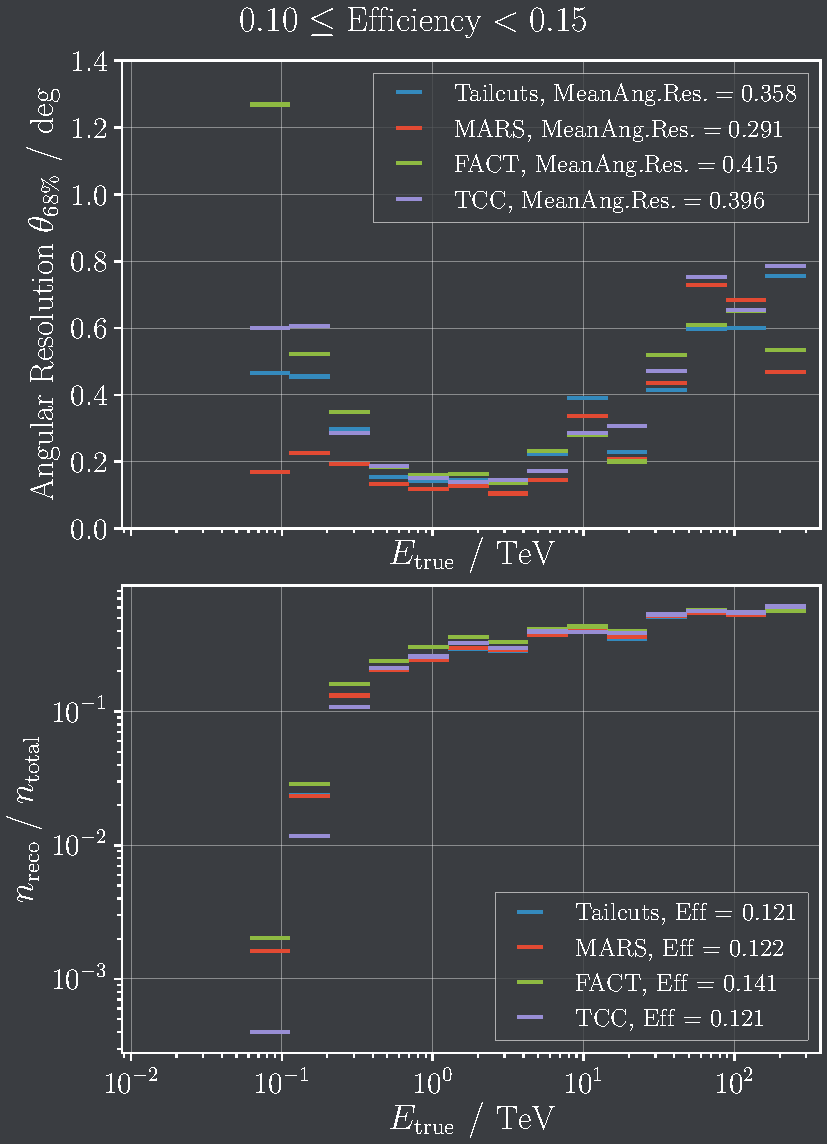
\includegraphics[height=0.8\textheight]{build/AR_Aeff_MST_0.10_0.15.pdf}
        \end{column}
        \begin{column}{0.48\textwidth}
            \centering
            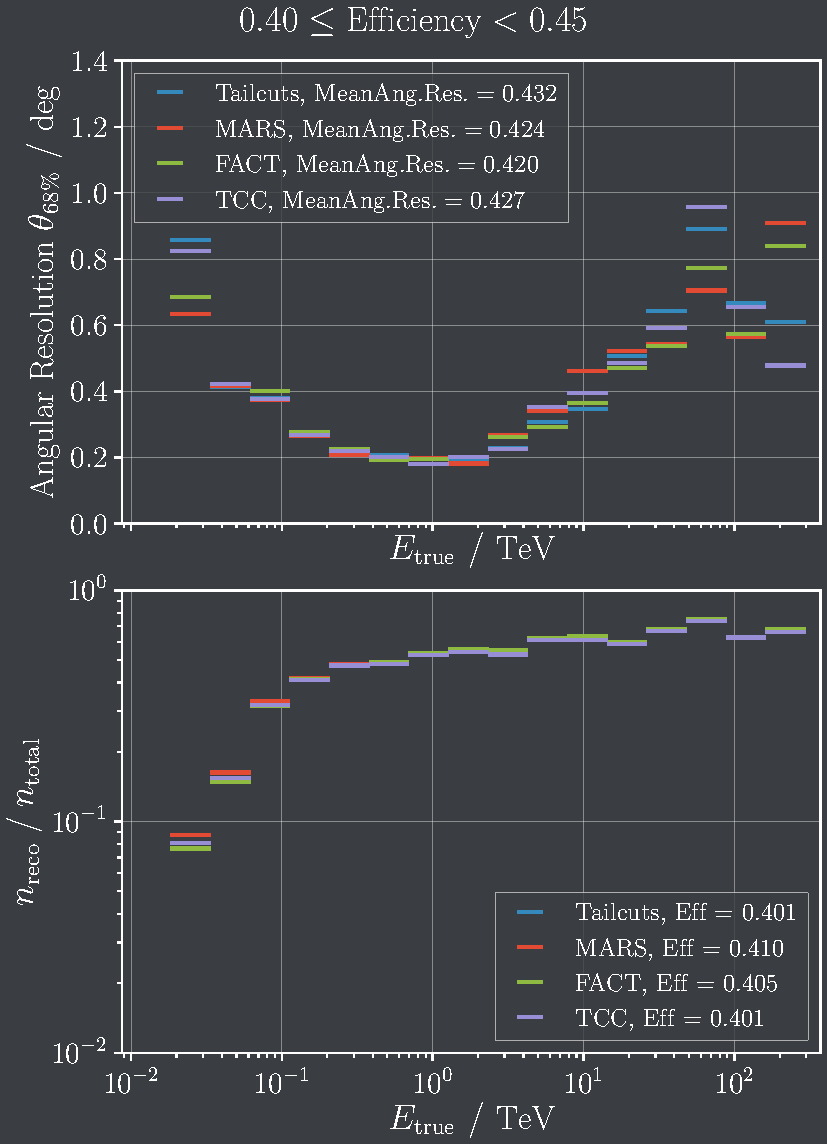
\includegraphics[height=0.8\textheight]{build/AR_Aeff_MST_0.40_0.45.pdf}
        \end{column}
    \end{columns}
\end{frame}

\begin{frame}{Efficiency vs. Angular Resolution}
    \centering
    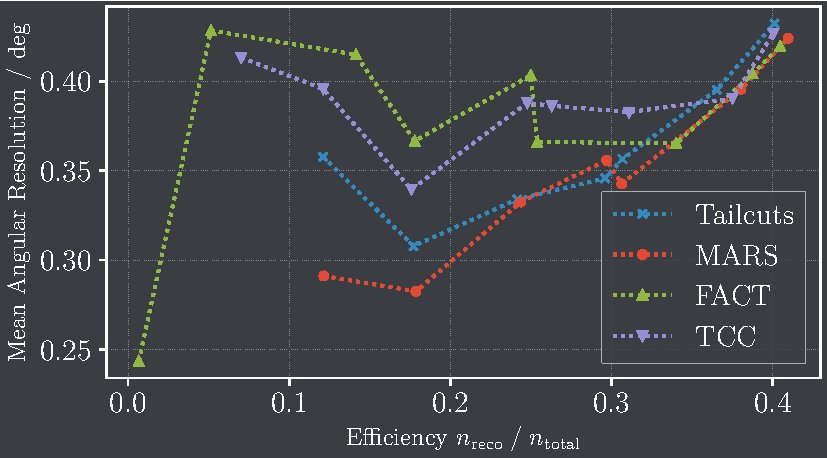
\includegraphics[width=0.75\textwidth]{build/ar_vs_eff.pdf}
\end{frame}

\begin{frame}{Evaluation Metrics}
    \begin{minipage}{0.48\textwidth}
        \begin{align*}
            \tpr &= \frac{\tp}{\tp + \fn} \\
            \tnr &= \frac{\tn}{\tn + \fp} \\
            \fnr &= \frac{\fn}{\fn + \tp} \\
            \acc &= \frac{\tp + \tn}{\tp + \fp + \tn + \fn} \\
            \ba &= \frac{\tpr + \tnr}{2}
        \end{align*}
    \end{minipage}
    \begin{minipage}{0.48\textwidth}
        \ifthenelse{\equal{\theme}{\string 1}}
            {% use dark theme
            \begin{table}
                \centering
                \begin{tabular}{r l c c}
                    & & \multicolumn{2}{c}{Prediction} \\
                    & & positive & negative \\
                    \parbox[t]{2mm}{\multirow{2}{*}{\rotatebox[origin=c]{90}{Label}}} &  pos. & \colorbox{darkmode!92!white}{True Positive ($\tp$)} & False Negative ($\fn$) \\
                    & neg. & False Positive ($\fp$) & \colorbox{darkmode!92!white}{True Negative ($\tn$)} \\
                \end{tabular}
            \end{table}%
            }
            {% use light theme
            \begin{table}
                \centering
                \begin{tabular}{r l c c}
                    & & \multicolumn{2}{c}{Prediction} \\
                    & & positive & negative \\
                    \parbox[t]{2mm}{\multirow{2}{*}{\rotatebox[origin=c]{90}{Label}}} &  pos. & \colorbox{white!92!black}{True Positive ($\tp$)} & False Negative ($\fn$) \\
                    & neg. & False Positive ($\fp$) & \colorbox{white!92!black}{True Negative ($\tn$)} \\
                \end{tabular}
            \end{table}%
            }
    \end{minipage}
\end{frame}

\begin{frame}{Metrics: \texttt{TailcutsImageCleaner}}
    \centering
    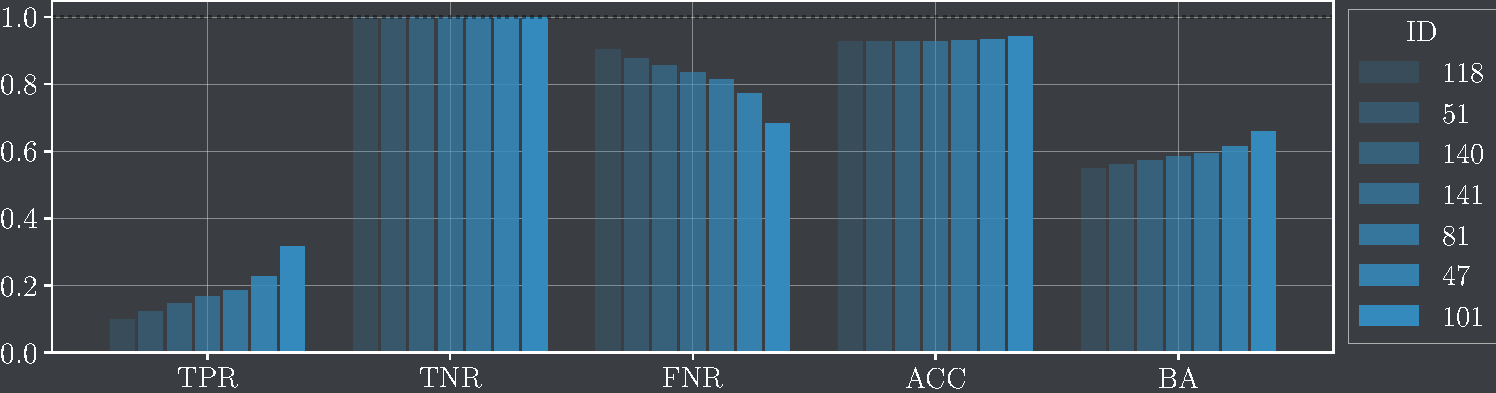
\includegraphics[width=0.9\textwidth]{build/metrics_tailcuts.pdf}
\end{frame}

\begin{frame}{Metrics: \texttt{MARSImageCleaner}}
    \centering
    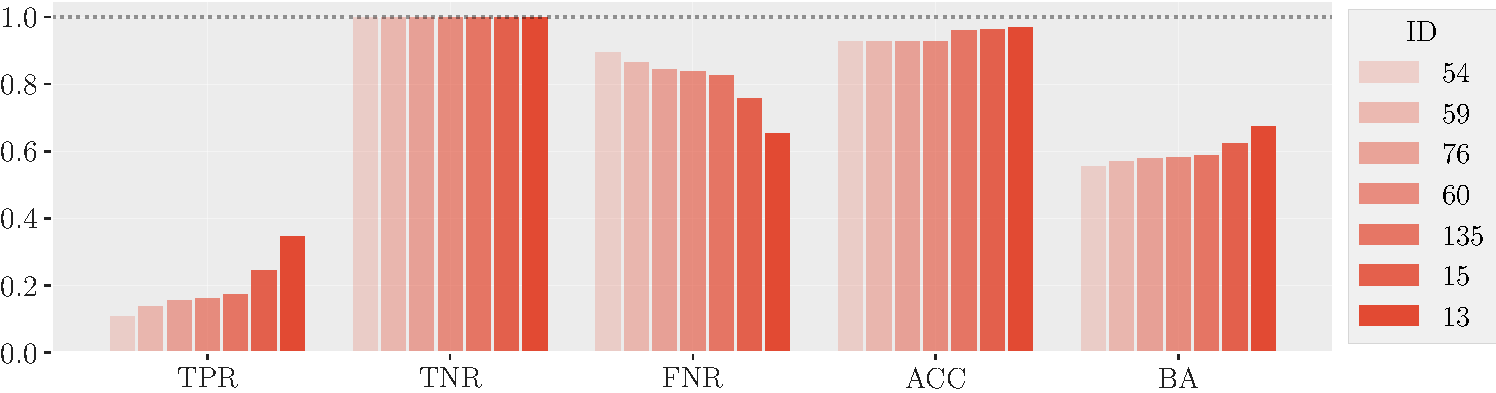
\includegraphics[width=0.9\textwidth]{build/metrics_mars.pdf}
\end{frame}

\begin{frame}{Metrics: \texttt{FACTImageCleaner}}
    \vspace{-0.355cm}
    \centering
    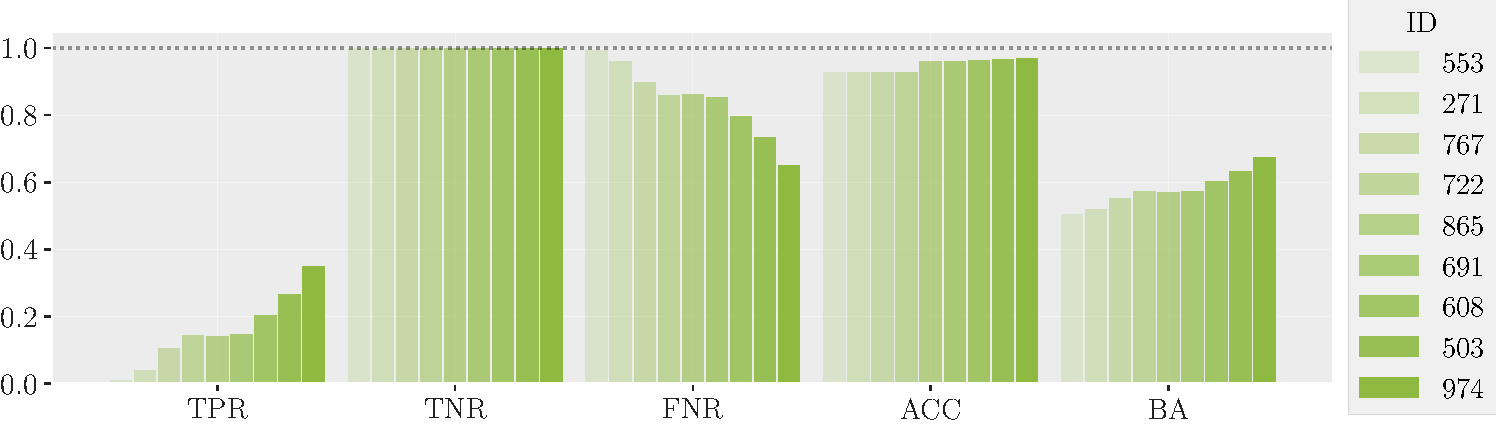
\includegraphics[width=0.9\textwidth]{build/metrics_fact.pdf}
\end{frame}

\begin{frame}{Metrics: \texttt{TimeConstraintImageCleaner}}
    \vspace{-0.15cm}
    \centering
    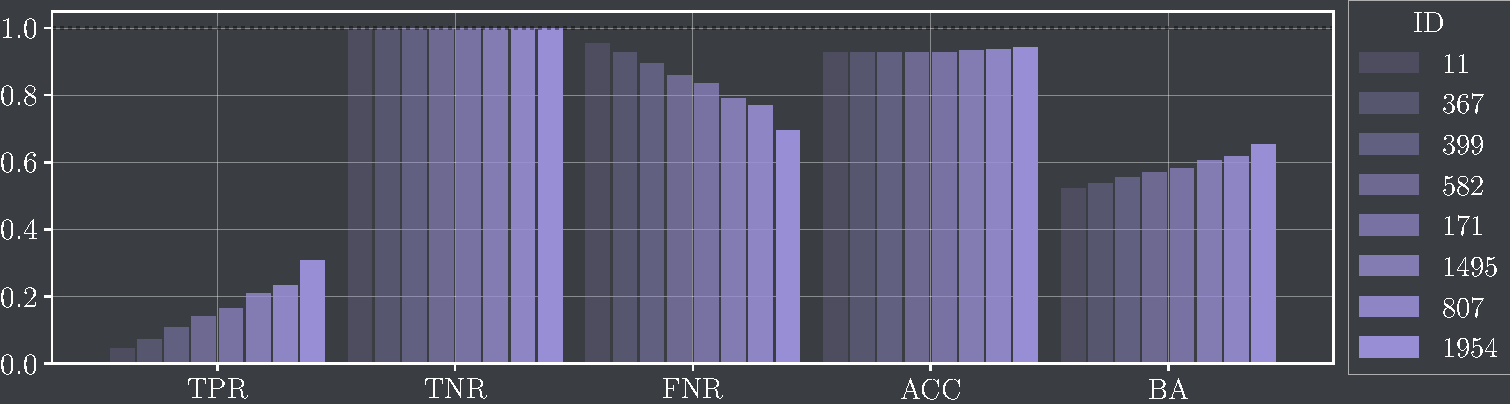
\includegraphics[width=0.9\textwidth]{build/metrics_tcc.pdf}
\end{frame}

\begin{frame}{Performance Compared to the Default Settings}
    \centering
    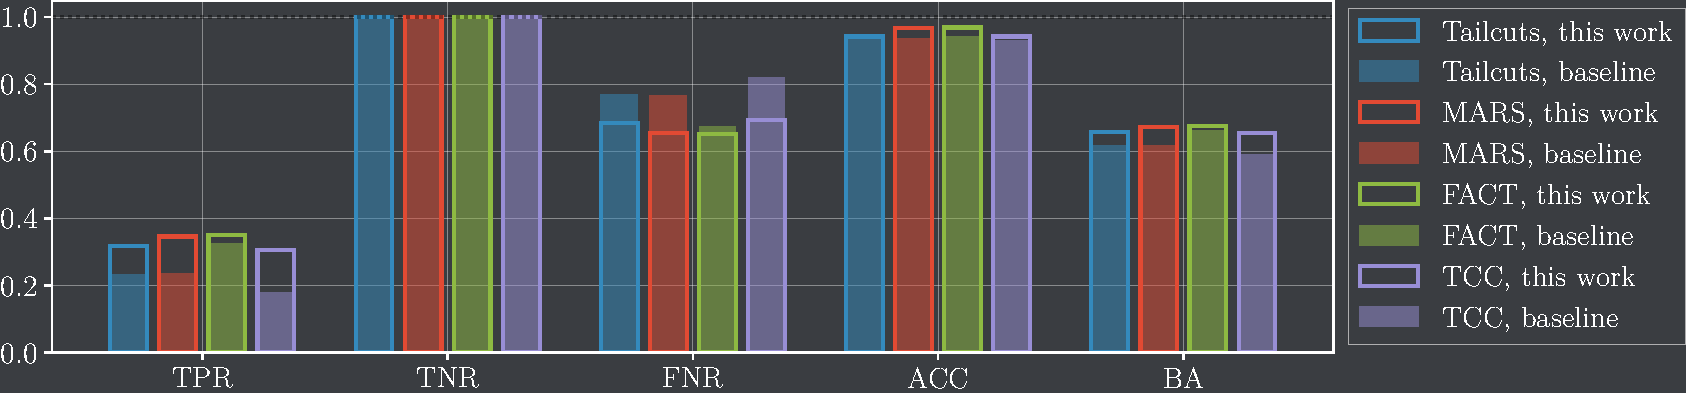
\includegraphics[width=0.9\textwidth]{build/metrics_baseline.pdf}
\end{frame}

\begin{frame}{Comparison of the Cleaning Algorithms}
    \centering
    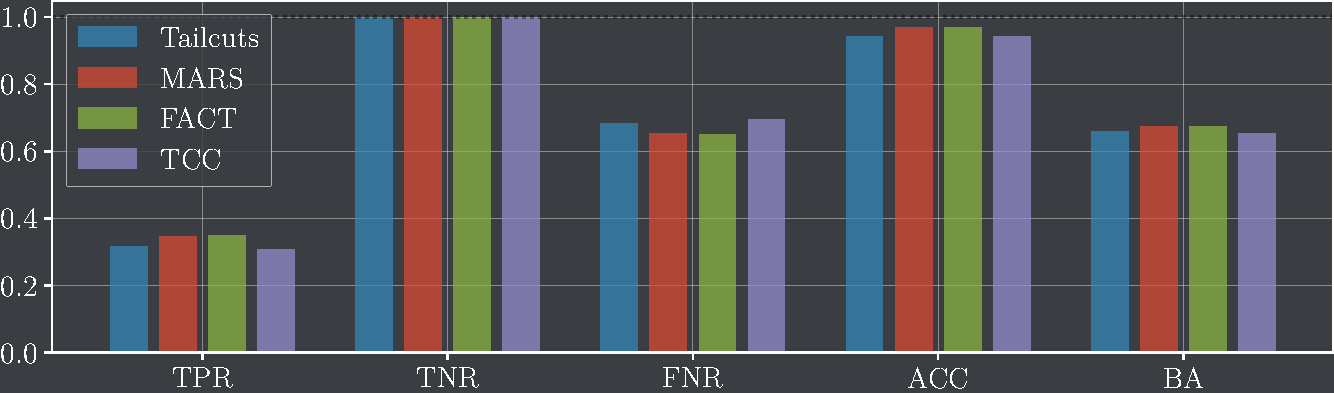
\includegraphics[width=0.9\textwidth]{build/metrics_all.pdf}
\end{frame}